\subsection*{2.1}
  % Implement the CE-CC amplifier shown below:
    \begin{figure}[h!]
        \centering
        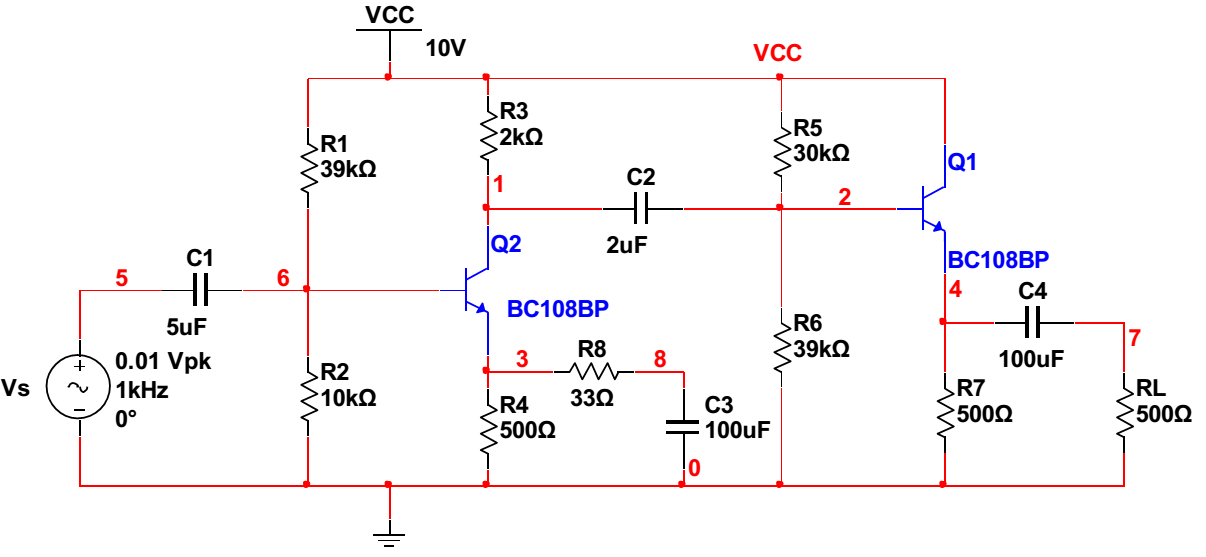
\includegraphics[width=13cm]{fig2-1.png}
        \captionof{figure}{The CE-CC amplifier to be implemented in Task 2.1}
    \end{figure}    

\subsection*{2.2}
  % Using  proper  simulation  techniques,  determine  the  following  parameters  of  the  circuit:
  \subsection*{(i) Midband voltage gain}

	\begin{figure}[h]
        \centering
        \begin{subfigure}[h]{0.5\textwidth}
                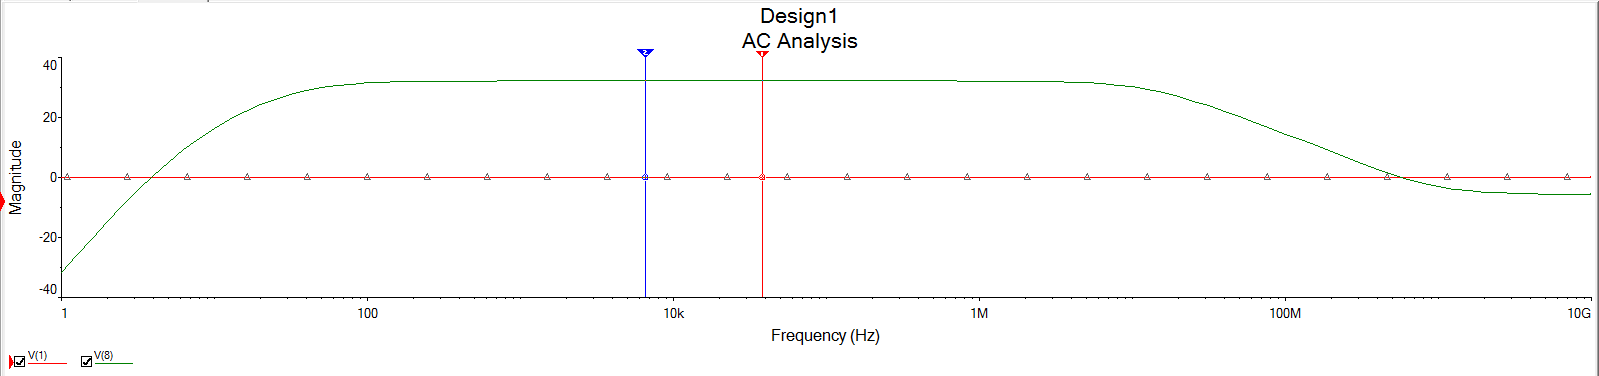
\includegraphics[width=\textwidth]{Task2_1A.png}
                \label{fig:HJÖRLEIFUR}
        \end{subfigure}
        \begin{subfigure}[h]{0.2\textwidth}
                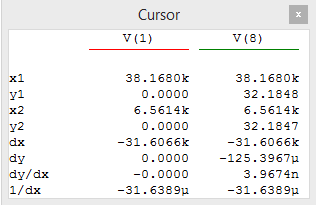
\includegraphics[width=\textwidth]{Task2_1B.png}
                \label{fig:LÁRUS}
        \end{subfigure}
        \captionof{figure}{AC analysis of circuit in figure X:Finding the midband gain}
	\end{figure}

    By using AC analysis in $MultiSim$ to determine the midband gain.
    By finding the output and input decibel at the midband and changing them to V/V, then determine the midband gain

   	From figure X hence the decibel for the output voltage is:
   	$$ V_{0} = 32.1848 dB $$ 
   	and the decibel for the input voltage is:
   	$$ V_{i} = 0 dB $$

   	$$ 20 \cdot log{\ V_{0} } = 32.1848 dB \rightarrow V_{0} = 40.66\  \frac{V}{V} $$
   	$$20 \cdot log{\ V_{i} } = 0  \rightarrow V_{i}= 1$$
   	$$A_{M} = \frac{V_{0}}{V_{i}} =\ 40.66 \ \frac{V}{V} $$


	\subsection*{(ii) Input resistance}
    \begin{figure}[h!]
        \centering
        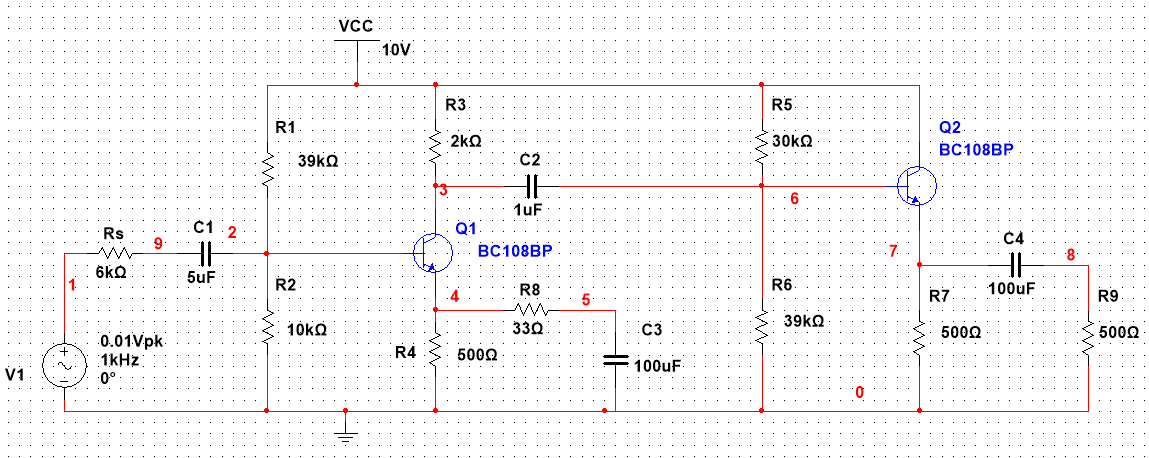
\includegraphics[width=13cm]{Task2_2C.png}
        \captionof{figure}{}
    \end{figure}  

	\begin{figure}[h]
        \centering
        \begin{subfigure}[h]{0.5\textwidth}
                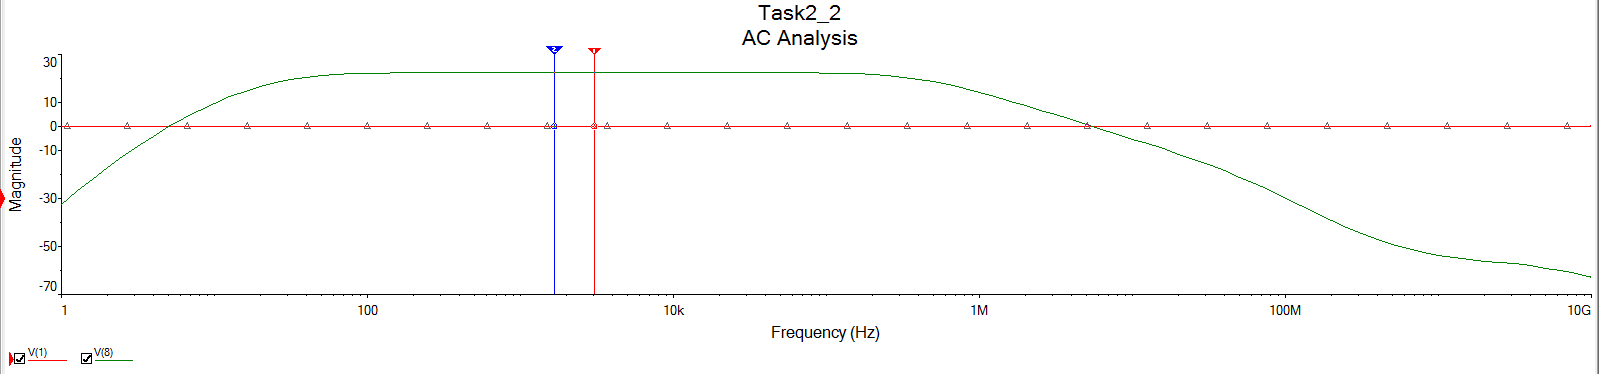
\includegraphics[width=\textwidth]{Task2_2A.png}
                \label{fig:}
        \end{subfigure}
        \begin{subfigure}[h]{0.2\textwidth}
                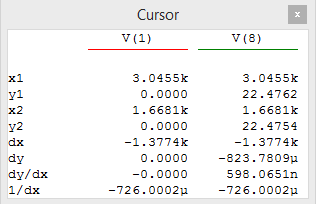
\includegraphics[width=\textwidth]{Task2_2B.png}
                \label{fig:}
        \end{subfigure}
        \captionof{figure}{}
	\end{figure}

	By adding a $R_{s}$ in the circuit we can find $R_{in}$.

	$$ A_{M2} = A_{M1} \cdot \frac{R_{in}}{R_{in} + R_{s}} \rightarrow R_{in} = \frac{R_{s}}{\frac{A_{M1}}{A_{M2}}-1} $$
	
	$$R_{in} = \frac{6\ kHz}{\frac{40.66}{18.19}-1} = 4857.14 \Omega \ $$ \\

 	\subsection*{(iii) Output resistance}

	\begin{figure}[h!]
	    \centering
	    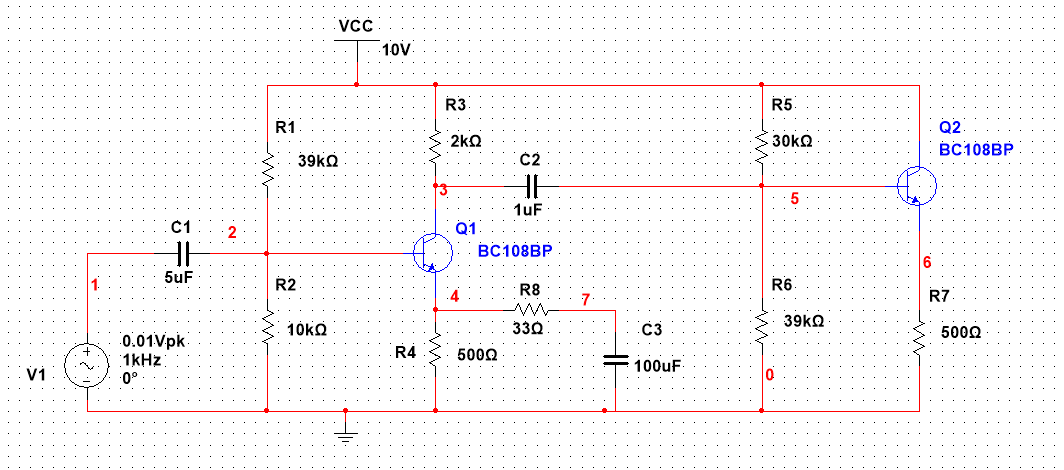
\includegraphics[width=13cm]{Task2_3C.png}
	    \captionof{figure}{}
	\end{figure}  

	\begin{figure}[h!]
	    \centering
	    \begin{subfigure}[h]{0.5\textwidth}
	            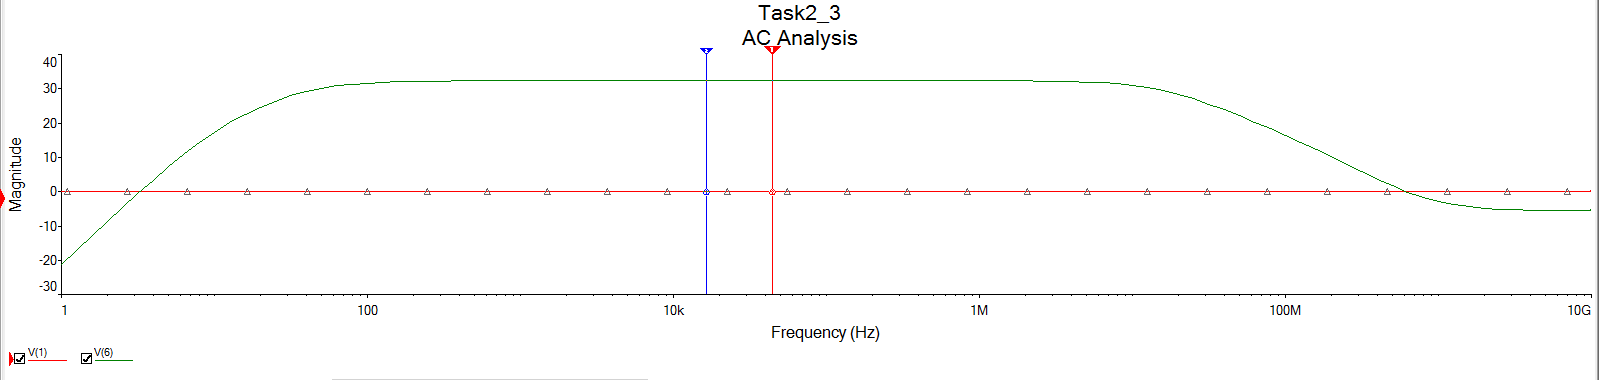
\includegraphics[width=\textwidth]{Task2_3A.png}
	            \label{fig:}
	    \end{subfigure}
	    \begin{subfigure}[h]{0.2\textwidth}
	            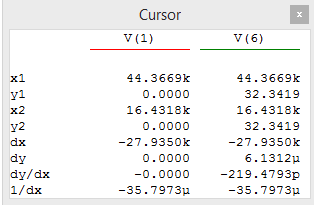
\includegraphics[width=\textwidth]{Task2_3B.png}
	            \label{fig:}
	    \end{subfigure}
	    \captionof{figure}{}
	\end{figure}

	By removing the load resistor and find the midband gain then determine the output resistor.

	$$A_{M1} = A_{M3} \cdot \frac{R_{L}}{R_{L} + R_{out}} \rightarrow R_{out} = R_{L} \cdot (\frac{A_{M3}}{A_{M1} - 1})  $$
	$$R_{out} = 500 \cdot (\frac{41.40}{40.66}-1) = 9.18\ \Omega$$ \\


	\subsection*{(iv) Lower 3dB frequency}

	\begin{figure}[h!]
	    \centering
	    \begin{subfigure}[h]{0.5\textwidth}
	            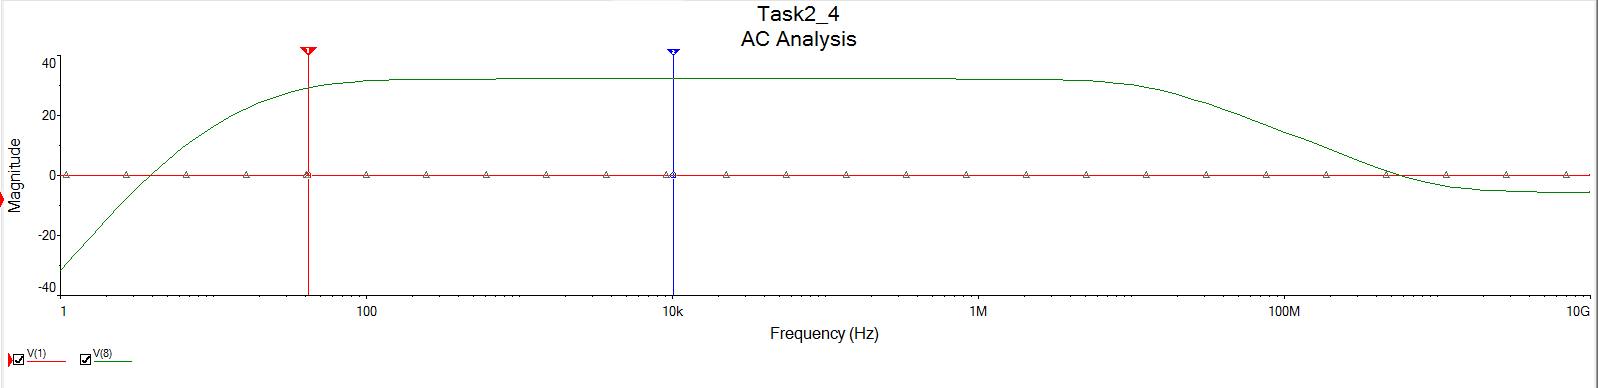
\includegraphics[width=\textwidth]{Task2_4A.png}
	            \label{fig:}
	    \end{subfigure}
	    \begin{subfigure}[h]{0.2\textwidth}
	            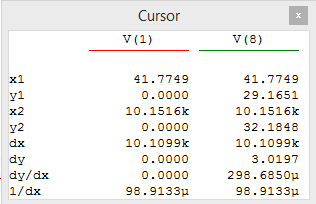
\includegraphics[width=\textwidth]{Task2_4B.png}
	            \label{fig:}
	    \end{subfigure}
	    \captionof{figure}{}
	\end{figure}
	
	\subsection*{(v) Upper 3dB frequency}

	\begin{figure}[h!]
	    \centering
	    \begin{subfigure}[h]{0.5\textwidth}
	            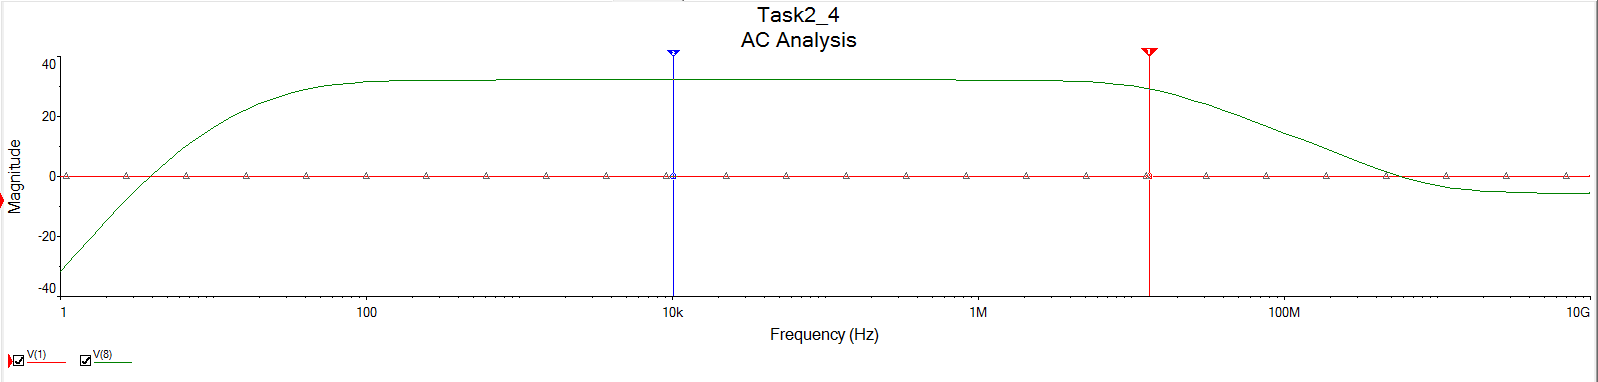
\includegraphics[width=\textwidth]{Task2_5A.png}
	            \label{fig:}
	    \end{subfigure}
	    \begin{subfigure}[h]{0.2\textwidth}
	            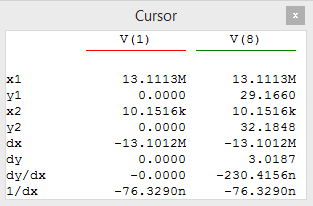
\includegraphics[width=\textwidth]{Task2_5B.png}
	            \label{fig:}
	    \end{subfigure}
	    \captionof{figure}{}
	\end{figure}
	asd




\subsection*{2.3}
  % Summarize  the  circuit  parameters  in  a  table  and  attach  relevant  plots.  Explain  the
  % simulation techniques that you exploited.
  